\documentclass{beamer}
\usepackage[utf8]{inputenc}

\usepackage[orientation=landscape,size=a0,scale=1.4,debug]{beamerposter}
\usepackage{hyperref}
\usetheme{Boadilla}
\usecolortheme{rose}

% biblatex (requires biber; sudo pacman -S biber)
\usepackage[style=authoryear-ibid]{biblatex} % biblatex
\addbibresource{"./content/bib/bib1.bib"}
\addbibresource{"./content/bib/bib2.bib"}

\usepackage{graphicx}
\graphicspath{ {./content/img/} }

\title[NEXTGEN]{NEXTGEN}
\subtitle{The \textit{\href{https://cryptolog.io}{Secret} Calculating} Technology}
\author[\href{https://nextgen.abdn.ac.uk}{nextgen.abdn.ac.uk} or \href{https://cryptolog.io}{cryptolog.io}]{George Onoufriou, Paul Mayfield, Georgios Leontidis}
\date{\today}

\begin{document}

  \begin{frame}
    \maketitle
    \begin{columns}
      \begin{column}{0.3\textwidth}
        \begin{block}{Fully Homomorphic Encryption as a Service}
          Despite the ever increasing prevalence of monitoring, tracking, and sensing, generating more data than ever before, we currently are unable to process this data in many circumstances. In some industries and settings this inability to process data arises from the sensitivity or indeed perceived sensitivity of the data that would otherwise be required to train or make use of state-of-the-art deep learning models. Other scenarios where data could not be processed would also include a lack of expertise being available, in particular for smaller entities such as farms, start-ups, etc. \\
          We propose and show in practice how fully homomorphic encryption as a service (\ref{fig:pipeline}) can be used to both protect the privacy and security of data owners, while allowing third parties to be called upon for data processing itself without any ability to decrypt \autocite{gentry2009fully} and subsequently making it impossible for data to be compromised even by quantum decryption thanks to FHE using the ring learning with errors problem, instead of plain prime factorization in most non-FHE encryption.
        \end{block}
      \end{column}
      \begin{column}{0.35\textwidth}
        \begin{block}{Fully Homomorphically Encrypted Pipeline}
          \begin{figure}
            \centering
            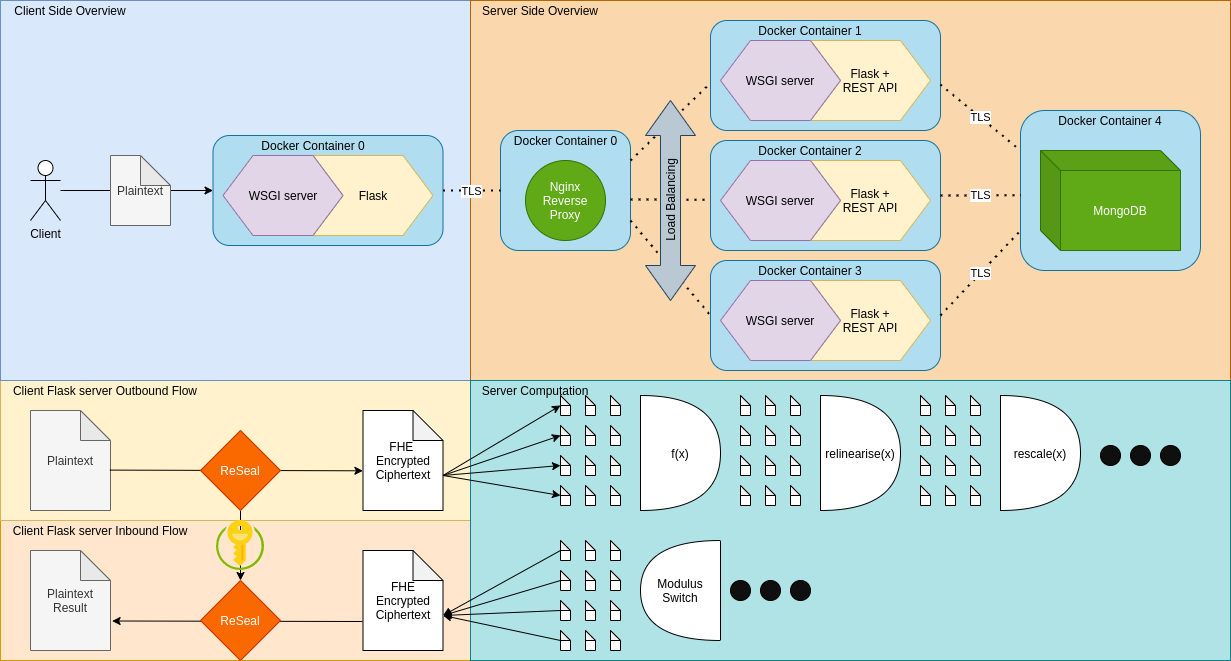
\includegraphics[width=\textwidth]{nextgen.png}
            \caption{Our server-client based pipeline and API for application and evaluation of FHE at some scale.}
            \label{fig:pipeline}
          \end{figure}
        \end{block}
      \end{column}
      \begin{column}{0.3\textwidth}
        \begin{block}{About our pipeline}
          To both evaluate, and implement FHE deep learning in practice, we decided to create a two part system.
          One local on-site edge device that serves as a standalone data wrangler, encryptor, and private key holder. This edge device is capable of obtaining the latest and most performant deep neaural network from our offsite archive, and using this to predict locally/ on-site albeit in a much diminished manner due to the naturally lower specification of an edge device. \\
          This device can also serve as a gateway for encrypted ciphertexts without their private keys, to go to an arbitrary backend server for much more intensive processing, which would require more performant hardware, while making it impossible for this backend/ off-site server to garner any information from this ciphertext being that it is undecryptable at any point offsite.
          Further to this both on-site and off-site servers expose both a web REST API and web app functionality to make it easy to use, while also creating an expandable interface and realistic scenarios for encrypted deep learning as a service to be evaluated properly.
        \end{block}
      \end{column}
    \end{columns}

    \begin{columns}
      \begin{column}{0.6\textwidth}
        \begin{block}{Fully Homomorphic Encryption Compatible Simple 1D CNN Computational Graph}
          \begin{figure}
            \centering
            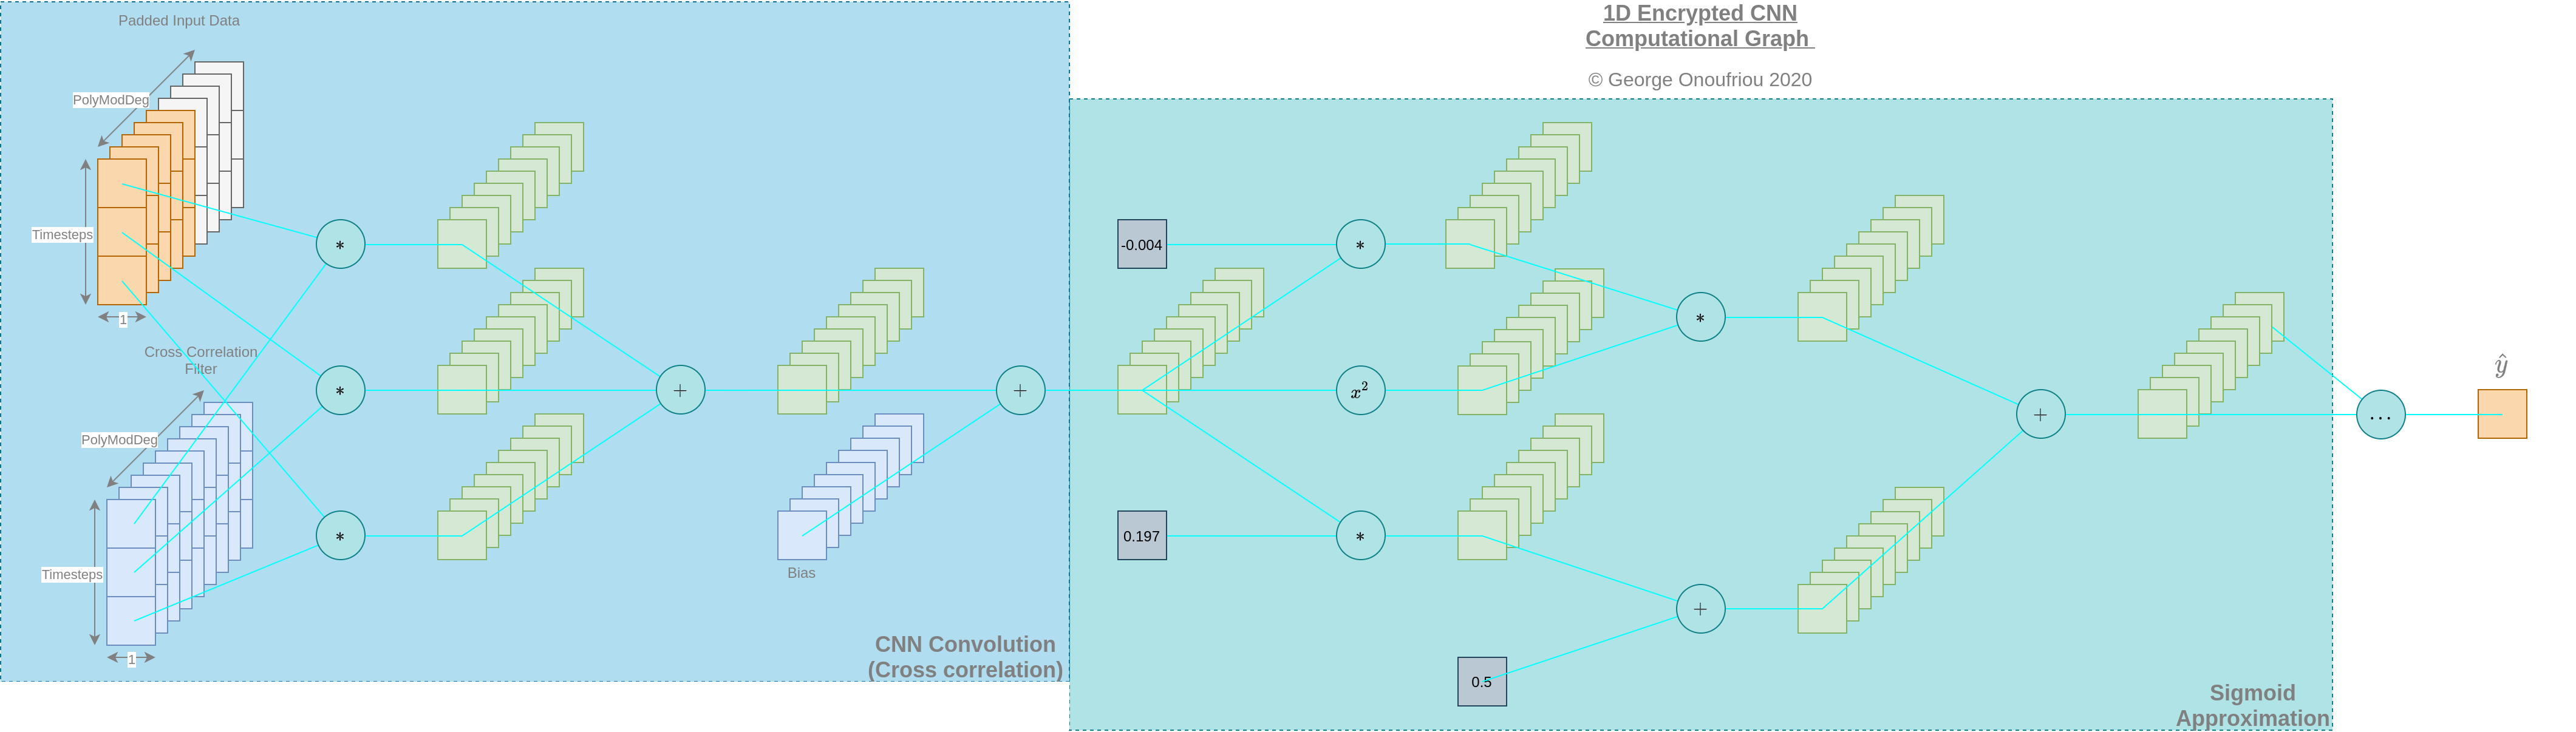
\includegraphics[width=\textwidth]{encrypted_cnn.png}
            \caption{FHE Compatible 1D CNN computational graph used to interchange space and time so historic milk yield and feeding cycles can be used to predict future yield while still using short computational depths of CNNs.}
            \label{fig:computational_graph}
          \end{figure}
        \end{block}
      \end{column}
      \begin{column}{0.35\textwidth}
        \begin{block}{Combining Deep Learning and Fully Homomorphic encryption}
          Deep Learning has become state-of-the-art in many machine learning tasks such as; image recognition, and classification; time series prediction, and sequence generation; self driving, and autonomous robotics. Thus since the majority of data desired to be processed is in tabular, and time series forms, or image, and video form, it only makes sense that to prove the applicability of FHE to computing this data that it should be evaluated and used in conjunction with deep learning i.e the state-of-the-art in these types of problems. \\
          We used the Cheon, Kim, Kim and Song (CKKS) \autocite{ckks} FHE encryption scheme, which is a form of FHE that allows it to operate on floating point numbers, which are the required type for deep learning which usually operates in the range 0-1. However all libraries available at this time are written in much lower level languages such as C++ compared to most deep learning frameworks which operate in python. To merge the two we had to create our own open source abstraction library and bindings to allow us to use CKKS FHE in python and at some scale. We also had to make sure neural networks in particular activation functions were compatible with FHE, since the only standard operation FHE cannot do is division of ciphertexts. Thus instead of sigmoid which includes division (Eq:\ref{sigmoid}) we used a close approximation (Eq:\ref{sigmoid_approx}) in the 1D CNN space as time equation \ref{cnn_activation}.
        \end{block}
      \end{column}
    \end{columns}

    \begin{columns}
      \begin{column}{0.3\textwidth}
        \begin{block}{FHE Compatibility and Deep Learning Equation Summary}
          \begin{equation}
            \label{sigmoid}
            \sigma(x) = \frac{1}{1+e^{-x}}
          \end{equation}
          \begin{equation}
            \label{sigmoid_approx}
            \sigma(x) \approx 0.5 + 0.197x + -0.004x^3
          \end{equation}
          \begin{equation}
            \label{cnn_activation}
            a^{<t>}=\sigma(w_{i}^{<t>}x^{<t>}+b_i^{<t>})
          \end{equation}
          \begin{equation}
            \label{gradient}
            \frac{df}{d\sigma} = (1-\sigma(x)) * \sigma(x)
          \end{equation}
          \begin{equation}
            \label{weight_update}
            % learning rate
            w_i^{j+1<t>} = w_i^{j<t>} - (l * \frac{df}{dw_i^{j<t>}})
          \end{equation}
        \end{block}
      \end{column}
      \begin{column}{0.3\textwidth}
        \begin{block}{Future Work}
          This projects focus was on proving that FHE could be used in practice, and at some scale. However we have begun and would like to in future continue working on  solving problems such as:
          \begin{itemize}
            \item Training neural networks, including calculating gradients (Eq:\ref{gradient}), and weight updates while encrypted (Eq:\ref{weight_update}).
            \item Utilizing parallel compute on the GPU to accelerate computation.
            \item Improving on the efficiency and optimize FHE deep learning.
          \end{itemize}
        \end{block}
      \end{column}
      \begin{column}{0.3\textwidth}
        \begin{block}{References}
          \printbibliography
        \end{block}
      \end{column}
    \end{columns}
  \end{frame}
\end{document}
